\section{Задание №7}

\begin{enumerate}
        \item Методом случайного поиска найти минимальное значение функции
$
        f
$ 
        на множестве 
$
        A = \{x_1, x_2 : x_1^2 + x_2^2 \leqslant 1\}
$
        , т.е.
$
        y = \min\limits_{x \in A} f(x)
$
        , где 
$$
        f(x) = x_1^3\sin\left(\frac{1}{x_1}\right) +10x_1 x_2^4\cos\left(\frac{1}{x_2}\right)
$$
        при $x_1 \neq 0$ и $x_2 \neq 0$, функция доопределяется по непрерывности при $x_1 = 0$ или $x_2 = 0$.
        
        \item Методом имитации отжига найти минимальное значение функции Розенброка $g$ в пространстве $\R^2$, где 
$$
        g(x) = (x_1-1)^2+100(x_2-x_1^2)^2.
$$

        \item Оценить точность. Сравнить результаты со стандартными методми оптимизации.
\end{enumerate}


\subsection{Метод случайного поиска}

Алгоритм поиска заключается в следующем: мы будем генерировать случайные величины, равномерно распределеные на единичной окружности, а затем сравним значения функции в этих точках и найдем среди них наименьшее.

Для начала предложим способ генерации таких случайных величин. Воспользуемся методом перехода в полярные координаты. Совместная плотность распределения случайных величин $x_1$, $x_2$ равна
$$
        \rho_{x_1,\,x_2}(x_1,\,x_2)
        =
        \begin{cases}
\frac{1}{\pi},
&
\mbox{ при $x_1^2 + x_2^2 \leqslant 1$,}
\\
0,
&
\mbox{ иначе.}
        \end{cases}
$$
Тогда
$$
        \p((x_1,\,x_2)^\T \in A)
=
        \iint\limits_{x_1^2 + x_2^2 \leqslant 1} \frac{1}{\pi}\,dxdy
=
        \left\{
\begin{aligned}
        &\; x_1 = r \cos\varphi, \\
        &\; x_2 = r \sin\varphi, \\
        &\; 0 \leqslant r \leqslant 1, \\
        &\; 0 \leqslant \varphi \leqslant 2\pi
\end{aligned}
        \right\}
=
        \frac{1}{\pi}\int\limits_{0}^{1}r\,dr \int\limits_0^{2\pi}\,d\varphi
=
        \int\limits_0^1 dr^2 \int\limits_0^{2\pi} \frac{1}{2\pi}\,d\varphi.
$$
В правой части последнего равенства получили получилось произведение двух интегралов. Первый показывает, что функция распределения случайной величины~$r$ на отрезке~$[0,\,1]$ равна $F_r(x) = x^2$; второй~--- что плотность распределения случайной величины~$\varphi$ на отрезке~$[0,\,2\pi]$ равна $\rho_\varphi(x) = \nicefrac{1}{2\pi}$. То есть
$$
        r = \sqrt{q}\mbox{, где }q \sim \mbox{U}[0,\,1],
\qquad
        \mbox{а }
        \varphi \sim \mbox{U}[0,\,2\pi].
$$

Теперь оценим точность предложенного алгоритма. Пусть $(x_1,\,x_2)$~--- точка минимума, полученная описанным выше методом, а $(x_1^*,\,x_2^*)$~--- реальная тока минимума. Тогда будем оценивать разность $|f(x_1,\,x_2) - f(x_1^*,\,x_2^*)|$. В этом нам поможет следующая теорема.

\begin{theorem}
        Пусть функция $f:\Omega \to \R$ непрерывно дифференцируема в выпуклой компактной области $\Omega$ пространства $\R^n$. Тогда $|f(x) - f(y)| \leqslant \sup\limits_{\xi\in\Omega}|\mbox{grad}\,f(\xi)|\cdot|x - y|$. 
\end{theorem}

Получается, что мы можем сделать следующее:
$$
      |f(x_1,\,x_2) - f(x_1^*,\,x_2^*)|
\leqslant
        \max\limits_{\xi_1^2 + \xi_2^2 \leqslant 1} |\mbox{grad}\,f(\xi_1,\,\xi_2)|\cdot\underbrace{\mbox{dist}((x_1,\,x_2)^\T,\,(x_1^*,\,x_2^*)^\T)}_{\delta}.  
$$
\begin{multline*}
        \left|
\frac{\partial f}{\partial x_1}
        \right|
=
        \left|
3x_1^2\sin\frac{1}{x_1} - x_1\cos\frac1{x_1} + 10x_2^4\cos\frac1{x_2}
        \right|
\leqslant \\ \leqslant
        3x_1^2\left|\sin\frac1{x_1}\right| + |x_1|\left|\cos\frac1{x_1}\right| + 10x_2^4\left|\cos\frac1{x_2}\right|
\leqslant
        3x_1^2 + |x_1| + 10x_2^4
= \\ =
        3x_1^2 + |x_1| + 10(1 - x_1^2)^2
\leqslant
        10x_1^4 - 17x_1^2 +  11
\leqslant
        11,
\end{multline*}
\begin{multline*}
        \left|
\frac{\partial f}{\partial x_2}
        \right|
=
        \left|
40x_1x_2^3\cos\frac1{x_2} + 10x_1x_2^2\sin\frac1{x_2}
        \right|
\leqslant
        40|x_1||x_2|\left|\cos\frac1{x_2}\right| + 10 |x_1|x_2^2\left|\sin\frac1{x_2}\right|
= \\ =
        10 |x_1| (1 - x_1^2)\left( 4\sqrt{1 - x_1^2} + 1 \right)
\leqslant
        50|x_1|(1 - x_1^2)
\leqslant
        19,\!245.
\end{multline*}
$$
        \Downarrow
$$
$$
        |f(x_1,\,x_2) - f(x_1^*,\,x_2^*)|
\leqslant
        \sqrt{11^2 + 19,\!245^2}\cdot\delta
\leqslant
        \underbrace{22,\!17}_{C}\delta.
$$

Оценка получена, но она зависит от того, насколько близко построенная нами случайная величина окажется к реальной точке минимума. Оценим вероятность того, что хотя бы одна случайная величина из $n$ окажется в $\delta$-окрестности искомой точки минимума. В худшем случае точка минимума может оказаться на границе множества~$A$ (в таком случае $\delta$-окрестность будет иметь минимальную площадь, а, значит, вероятность попадания туда равномерно распределенной случайной величины будет минимальной), поэтому оценивать будем вероятность вероятность попадания именно в граничную $\delta$-окрестность. Также учтем, что заданная функция $f$ является четной по переменной $x_2$, что говорит о наличии как минимум двух точек минимума, поэтому вероятность попадания в окрестности минимумов увеличивается в 2 раза.
$$
        p
\geqslant
        1 - \left( 1 - \frac{\arccos(2 - \frac{\delta^2}{2}) - 2\sin\left(\arccos(1 - \frac{\delta^2}{2})\right) + \pi\delta^2}{\pi}\right)^n
\approx
        1 - (1 - \delta^2)^n. 
$$

Теперь, мы можем определить сколько потребуется генераций случайной величины, чтобы найти минимум функции с заданной погрешностью и уровнем доверия. В рамках же задания мы пойдем обратным путем: мы будем вычислять погрешность, исходя из уровня доверия и количества генераций:
$$
        \varepsilon
=
        C\left( 1 - (1 - p)^{\frac{1}{n}} \right)^{\frac12}
\approx
        C\sqrt{\frac{p}{n}}
=
22,\!17\sqrt{\frac{p}{n}}.
$$

\begin{table}[h]
\begin{center}
\begin{tabular}{|c|c|c|}
\hline
Число генераций &
Результат  &
Погрешность
\\
\hline
$10^5$
&
$-1,\!286\;\;$
&
$0,\!0698$
\\
\hline
$10^6$
&
$-1,\!2879$
&
$0,\!0221$
\\
\hline
$10^7$
&
$-1,\!2882$
&
$0,\!007\;\;$
\\
\hline
$10^8$
&
$-1,\!2884$
&
$0,\!0022$
\\
\hline
\end{tabular}
\end{center}
\caption{Результат работы метода случайного поиска при различном количестве генераций при уровне доверия $p = 0,\!99$.}
\end{table}


\subsection{Метод имитации отжига}

Алгоритм основывается на имитации физического процесса, который происходит при кристаллизации вещества, в том числе при отжиге металлов. Предполагается, что атомы уже выстроились в кристалличекую решётку, но ещё допустимы переходы отдельных атомов из одной ячейки в другую. Предполагается, что процесс протекает при постепенно понижающейся температуре. Переход атома из одной ячейки в другую происходит с некоторой вероятностью, причём вероятность понижается с понижением температуры. Устойчивая кристаллическая решётка соответствует минимуму энергии атомов, поэтому атом либо переходит в состояние с меньшим уровнем энергии, либо остаётся на месте.

При помощи моделирования такого процесса ищется такая точка или множество точек, на котором достигается минимум числовой функции $g(x)$, где $x=(x_1,\,\ldots,\,x_m) \in X$. Решение ищется последовательным вычислением точек $x^0,\,x^1,\,\ldots$ пространства $X$; каждая точка, начиная с $x^1$, "<претендует"> на то, чтобы лучше предыдущих приближать решение. Алгоритм принимает точку $x^0$ как исходные данные. На каждом шаге алгоритм (который описан ниже) вычисляет новую точку и понижает значение величины (изначально положительной), понимаемой как "<температура">. Алгоритм останавливается по достижении точки, которая оказывается при температуре ноль.

Точка $x^{i+1}$ по алгоритму получается на основе текущей точки $x^i$ следующим образом. К точке $x_i$ применяется оператор $A$, который случайным образом модифицирует соответствующую точку, в результате чего получается новая точка $x^*$. Точка $x^*$ становится точкой $x^{i+1}$ с вероятностью $p(x^*,\,x^{i+1})$, которая вычисляется в соответствии с распределением Гиббса:
$$
        p(x^*\to x^{i+1}\,|\,x^i)
=
        \begin{cases}
1,
        &
\mbox{при $g(x^*) - g(x^i) < 0$,}
        \\
\exp\left(-\frac{g(x^*) - g(x^i)}{t_i}\right),
        &
\mbox{при $g(x^*) - g(x^i) \geqslant 0$}.
\end{cases}
$$

Здесь $t_i>0$~--- элементы произвольной убывающей, сходящейся к нулю положительной последовательности, которая задаёт аналог падающей температуры в кристалле. Скорость убывания и закон убывания могут быть заданы по желанию создателя алгоритма.

Алгоритм имитации отжига похож на градиентный спуск, но за счёт случайности выбора промежуточной точки должен попадать в локальные минимумы реже, чем градиентный спуск. Алгоритм имитации отжига не гарантирует нахождения минимума функции, однако при правильной политике генерации случайной точки в пространстве $X$, как правило, происходит улучшение начального приближения.

\clearpage
\begin{table}[t]
\begin{center}
\begin{tabular}{|c|c|c|}
\hline
Число генераций &
Результат 
\\
\hline
$10^2$
&
$6,\!1673\cdot10^{-6}$
\\
\hline
$10^3$
&
$1,\!2550\cdot10^{-7}$
\\
\hline
$10^4$
&
$2,\!8228\cdot10^{-8}$
\\
\hline
\end{tabular}
\end{center}
\caption{Результат работы метода имитации отжига.}
\end{table}

\begin{figure}[b]
        \noindent
        \centering
        {
                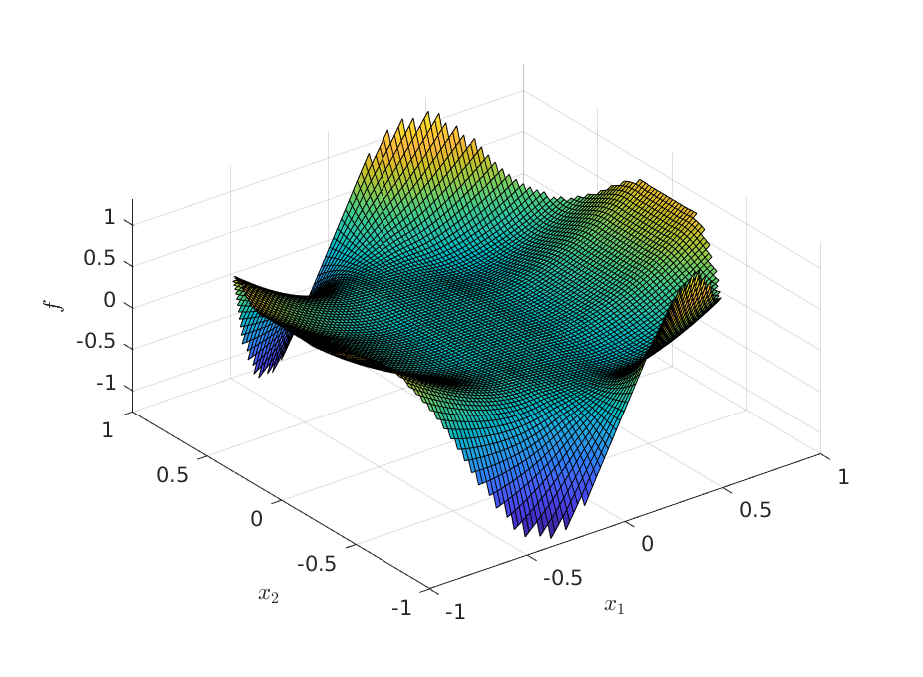
\includegraphics[width=120mm]{task_07/f_func.eps}
        }
        \caption{Внешний вид функции $f(x)$ на множестве $x_1^2 + x_2^2 \leqslant 1$. Видно, где достигается минимум и его примерное значение, поэтому предложенное решение не единственное. Действительно, из-за того, что минимум достигается на границе, мы могли сузить область случайного поиска, например, на граничную окружность.}
\end{figure}
\clearpage
\begin{figure}[t]
        \noindent
        \centering
        {
                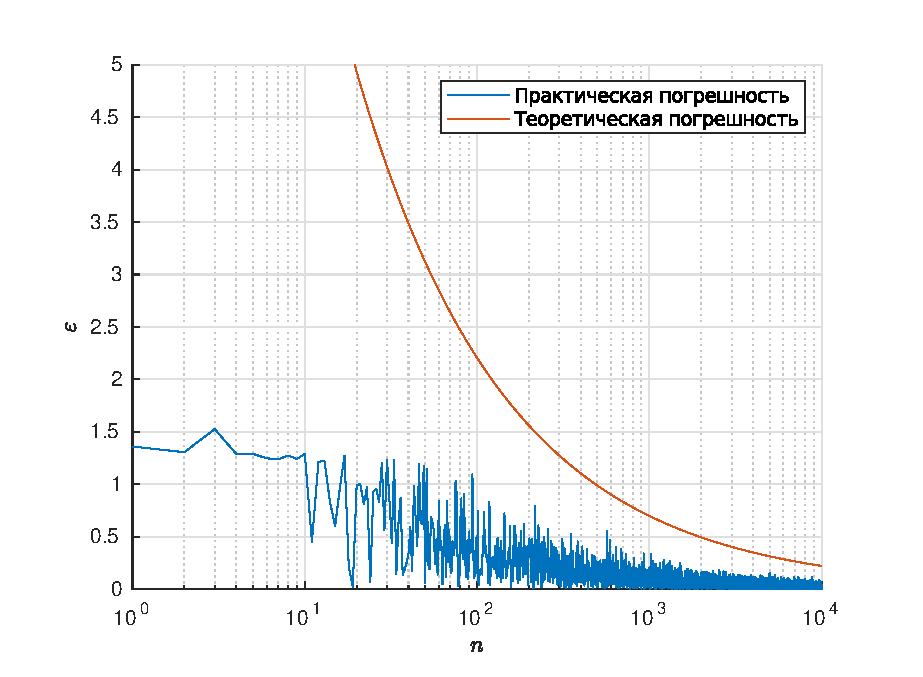
\includegraphics[width=120mm]{task_07/speed.eps}
        }
        \caption{Скорость сходимости метода случайного поиска и его ее верхняя оценка с уровнем доверия $p = 0,\!99$ для заданной функции $f(x)$. Для поиска практической погрешности было найдено реальное значение минимума, равное $-1,\!2885$, при помощи метода градиентного спуска.}
\end{figure}
\begin{figure}[b]
       \noindent
        \centering
        {
                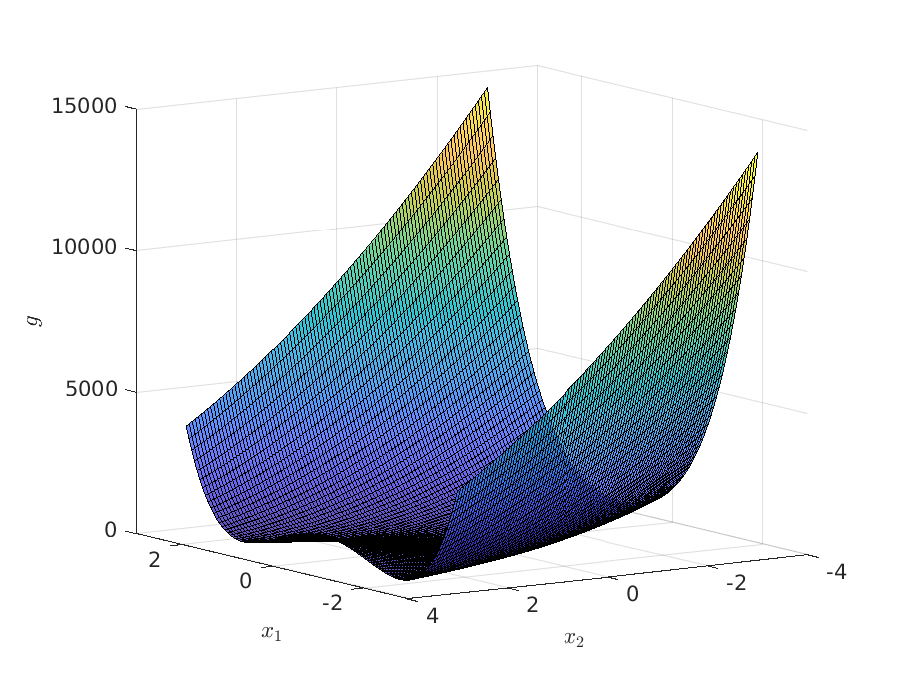
\includegraphics[width=120mm]{task_07/g_func.eps}
        }
        \caption{Внешний вид функции $g(x_1,\,x_2)$ на квадрате со стороной 3.}
\end{figure}